%!TEX TS-program = xelatex
%!TEX encoding = UTF-8 Unicode
% Awesome CV LaTeX Template for CV/Resume
%
% This template has been downloaded from:
% https://github.com/posquit0/Awesome-CV
%
% Author:
% Claud D. Park <posquit0.bj@gmail.com>
% http://www.posquit0.com
%
% Template license:
% CC BY-SA 4.0 (https://creativecommons.org/licenses/by-sa/4.0/)
%

%-------------------------------------------------------------------------------
% CONFIGURATIONS
%-------------------------------------------------------------------------------
% A4 paper size by default, use 'letterpaper' for US letter
\documentclass[11pt, a4paper]{awesome-cv}

% Allow Japanese fonts
\usepackage{xeCJK}
\setCJKmainfont{mplus-1m-thin} % for \rmfamily
\setCJKsansfont{mplus-1m-thin} % for \sffamily

% Allow embedding of images
\usepackage{graphicx}
\graphicspath{ {./resume/} }

% Configure page margins with geometry
\geometry{left=1.4cm, top=.8cm, right=1.4cm, bottom=1.8cm, footskip=.5cm}

% Specify the location of the included fonts
\fontdir[fonts/]

% Color for highlights
% Awesome Colors: awesome-emerald, awesome-skyblue, awesome-red, awesome-pink, awesome-orange
%                 awesome-nephritis, awesome-concrete, awesome-darknight
% \colorlet{awesome}{awesome-red}
% Uncomment if you would like to specify your own color
% \definecolor{awesome}{HTML}{CA63A8}
% \definecolor{awesome}{HTML}{7f24b3} % purple
% \definecolor{awesome}{HTML}{565be3} % blue
\definecolor{awesome}{HTML}{2429b5} % blue
% \definecolor{awesome}{HTML}{780a0a} % burgundy

% Colors for text
% Uncomment if you would like to specify your own color
% \definecolor{darktext}{HTML}{414141}
% \definecolor{text}{HTML}{333333}
% \definecolor{graytext}{HTML}{5D5D5D}
% \definecolor{lighttext}{HTML}{999999}

% Set false if you don't want to highlight section with awesome color
\setbool{acvSectionColorHighlight}{true}

% If you would like to change the social information separator from a pipe (|) to something else
\renewcommand{\acvHeaderSocialSep}{\quad\textbar\quad}


%-------------------------------------------------------------------------------
%	PERSONAL INFORMATION
%	Comment any of the lines below if they are not required
%-------------------------------------------------------------------------------
% Available options: circle|rectangle,edge/noedge,left/right
% \photo[rectangle,edge,right]{./examples/profile}
\name{Andrew J.}{Pierce}
\position{Engineering Manager{\enskip\cdotp\enskip}Software Architect}
\address{2928 Gray St. Oakton, VA 22124}

\mobile{703-967-1368}
\email{andrew.j.pierce@gmail.com}
\homepage{ajpierce.com}
\github{ajpierce}
\github{owap}
% \linkedin{posquit0}
% \gitlab{gitlab-id}
% \stackoverflow{SO-id}{SO-name}
% \twitter{@twit}
% \skype{skype-id}
% \reddit{reddit-id}
% \medium{madium-id}
% \googlescholar{googlescholar-id}{name-to-display}
%% \firstname and \lastname will be used
% \googlescholar{googlescholar-id}{}
% \extrainfo{extra informations}

% \quote{``Be the change that you want to see in the world."}


%-------------------------------------------------------------------------------
\begin{document}

% Print the header with above personal informations
% Give optional argument to change alignment(C: center, L: left, R: right)
\makecvheader[C]

% Print the footer with 3 arguments(<left>, <center>, <right>)
% Leave any of these blank if they are not needed
\makecvfooter
  {\today}
  {Andrew J. Pierce~~~·~~~Résumé}
  {\thepage}


%-------------------------------------------------------------------------------
%	CV/RESUME CONTENT
%	Each section is imported separately, open each file in turn to modify content
%-------------------------------------------------------------------------------
%-------------------------------------------------------------------------------
%	SECTION TITLE
%-------------------------------------------------------------------------------
\cvsection{Summary}


%-------------------------------------------------------------------------------
%	CONTENT
%-------------------------------------------------------------------------------
\begin{cvparagraph}

%---------------------------------------------------------
Positive and insightful leader and engineer with over a decade of experience growing startups into multi-million dollar organizations while delivering large, high-impact projects on time.
Seasoned AWS architect with an eye for resilient and cost-effective solutions.
Experienced public speaker and presenter comfortable with everything from large trade shows and hackathons to code reviews and tech talks with the team.
Polyglot who believes in using the best tool for the job.
Champion of processes and practices that yield compounding gains.
\end{cvparagraph}
\begin{figure}[h]
  \vspace*{-3mm}
  \centering
  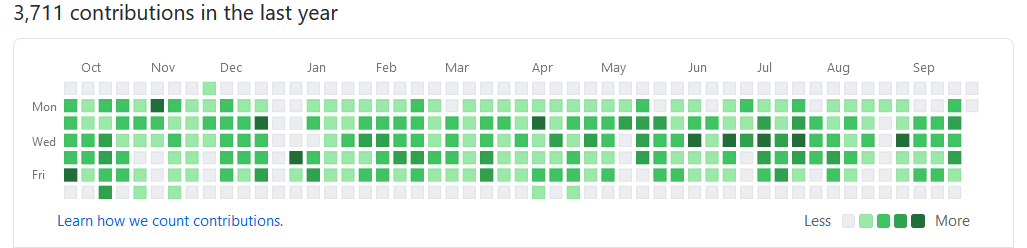
\includegraphics[width=0.8\textwidth]{github.png}
\end{figure}


%-------------------------------------------------------------------------------
%	SECTION TITLE
%-------------------------------------------------------------------------------
\cvsection{Work Experience}


%-------------------------------------------------------------------------------
%	CONTENT
%-------------------------------------------------------------------------------
\begin{cventries}

%---------------------------------------------------------
  \cventry
    {Software Architect} % Job title
    {Omnious. Co., Ltd.} % Organization
    {Seoul, S.Korea} % Location
    {Jun. 2017 - May. 2018} % Date(s)
    {
      \begin{cvitems} % Description(s) of tasks/responsibilities
        \item {Provisioned an easily managable hybrid infrastructure(Amazon AWS + On-premise) utilizing IaC(Infrastructure as Code) tools like Ansible, Packer and Terraform.}
        \item {Built fully automated CI/CD pipelines on CircleCI for containerized applications using Docker, AWS ECR and Rancher.}
        \item {Designed an overall service architecture and pipelines of the Machine Learning based Fashion Tagging API SaaS product with the micro-services architecture.}
        \item {Implemented several API microservices in Node.js Koa and in the serverless AWS Lambda functions.}
        \item {Deployed a centralized logging environment(ELK, Filebeat, CloudWatch, S3) which gather log data from docker containers and AWS resources.}
        \item {Deployed a centralized monitoring environment(Grafana, InfluxDB, CollectD) which gather system metrics as well as docker run-time metrics.}
      \end{cvitems}
    }

%---------------------------------------------------------
  \cventry
    {Co-founder \& Software Engineer} % Job title
    {PLAT Corp.} % Organization
    {Seoul, S.Korea} % Location
    {Jan. 2016 - Jun. 2017} % Date(s)
    {
      \begin{cvitems} % Description(s) of tasks/responsibilities
        \item {Implemented RESTful API server for car rental booking application(CARPLAT in Google Play).}
        \item {Built and deployed overall service infrastructure utilizing Docker container, CircleCI, and several AWS stack(Including EC2, ECS, Route 53, S3, CloudFront, RDS, ElastiCache, IAM), focusing on high-availability, fault tolerance, and auto-scaling.}
        \item {Developed an easy-to-use Payment module which connects to major PG(Payment Gateway) companies in Korea.}
      \end{cvitems}
    }

%---------------------------------------------------------
  \cventry
    {Software Engineer \& Security Researcher (Compulsory Military Service)} % Job title
    {R.O.K Cyber Command, MND} % Organization
    {Seoul, S.Korea} % Location
    {Aug. 2014 - Apr. 2016} % Date(s)
    {
      \begin{cvitems} % Description(s) of tasks/responsibilities
        \item {Lead engineer on agent-less backtracking system that can discover client device's fingerprint(including public and private IP) independently of the Proxy, VPN and NAT.}
        \item {Implemented a distributed web stress test tool with high anonymity.}
        \item {Implemented a military cooperation system which is web based real time messenger in Scala on Lift.}
      \end{cvitems}
    }

%---------------------------------------------------------
  \cventry
    {Game Developer Intern at Global Internship Program} % Job title
    {NEXON} % Organization
    {Seoul, S.Korea \& LA, U.S.A} % Location
    {Jan. 2013 - Feb. 2013} % Date(s)
    {
      \begin{cvitems} % Description(s) of tasks/responsibilities
        \item {Developed in Cocos2d-x an action puzzle game(Dragon Buster) targeting U.S. market.}
        \item {Implemented API server which is communicating with game client and In-App Store, along with two other team members who wrote the game logic and designed game graphics.}
        \item {Won the 2nd prize in final evaluation.}
      \end{cvitems}
    }

%---------------------------------------------------------
  \cventry
    {Software Engineer} % Job title
    {ShitOne Corp.} % Organization
    {Seoul, S.Korea} % Location
    {Dec. 2011 - Feb. 2012} % Date(s)
    {
      \begin{cvitems} % Description(s) of tasks/responsibilities
        \item {Developed a proxy drive smartphone application which connects proxy driver and customer.}
        \item {Implemented overall Android application logic and wrote API server for community service, along with lead engineer who designed bidding protocol on raw socket and implemented API server for bidding.}
      \end{cvitems}
    }

%---------------------------------------------------------
  \cventry
    {Freelance Penetration Tester} % Job title
    {SAMSUNG Electronics} % Organization
    {S.Korea} % Location
    {Sep. 2013, Mar. 2011 - Oct. 2011} % Date(s)
    {
      \begin{cvitems} % Description(s) of tasks/responsibilities
        \item {Conducted penetration testing on SAMSUNG KNOX, which is solution for enterprise mobile security.}
        \item {Conducted penetration testing on SAMSUNG Smart TV.}
      \end{cvitems}
      %\begin{cvsubentries}
      %  \cvsubentry{}{KNOX(Solution for Enterprise Mobile Security) Penetration Testing}{Sep. 2013}{}
      %  \cvsubentry{}{Smart TV Penetration Testing}{Mar. 2011 - Oct. 2011}{}
      %\end{cvsubentries}
    }

%---------------------------------------------------------
\end{cventries}

% \input{resume/honors.tex}
% \input{resume/presentation.tex}
% \input{resume/writing.tex}
% \input{resume/committees.tex}
%-------------------------------------------------------------------------------
%	SECTION TITLE
%-------------------------------------------------------------------------------
\cvsection{Education}


%-------------------------------------------------------------------------------
%	CONTENT
%-------------------------------------------------------------------------------
\begin{cventries}

%---------------------------------------------------------
  \cventry
    {Graduated \emph{Cum Laude}} % Degree
    {College of William \& Mary} % Institution
    {Williamsburg, VA} % Location
    {August 2005 - May 2009} % Date(s)
    {
      \begin{cvitems} % Description(s) bullet points
        \item {B.S. Computer Science}
        \item {B.A. Japanese Studies}
      \end{cvitems}
    }

%---------------------------------------------------------
\end{cventries}

% \input{resume/extracurricular.tex}


%-------------------------------------------------------------------------------
\end{document}
